\documentclass[usenames,dvipsnames,tikz]{standalone}
\usepackage{amsmath,amssymb}
\usepackage{xcolor}
\colorlet{tBlue}{RoyalBlue!35!Cerulean}
\colorlet{tRed}{Red}
\usepackage{tikz}
\usepackage{standalone}
\begin{document}
	
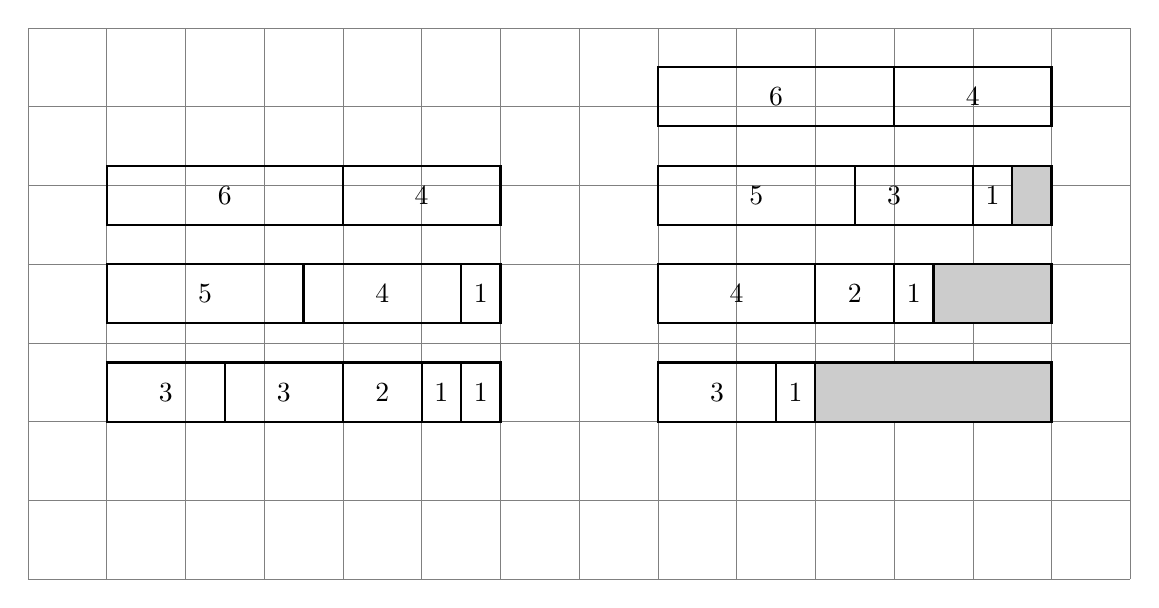
\begin{tikzpicture}
\draw [help lines] (-1,-2) grid (13,5);
% 1=0.1, 2=0.15, 3=0.2, 4=0.25, 5=0.3
% 6, 5, 4, 4, 3, 3, 2, 1, 1, 1.

% BPP
\draw [thick] (0,0) rectangle (5,0.75);
\draw [thick] (0,1.25) rectangle (5,2);
\draw [thick] (0,2.5) rectangle (5,3.25);

% Bottom row, 3, 3, 2, 1
\draw [thick] (1.5,0) -- (1.5,0.75);
\draw [thick] (3,0) -- (3,0.75);
\draw [thick] (4,0) -- (4,0.75);
\draw [thick] (4.5,0) -- (4.5,0.75);
\node at (0.75, 0.375) {3};
\node at (2.25, 0.375) {3};
\node at (3.5, 0.375) {2};
\node at (4.25, 0.375) {1};
\node at (4.75, 0.375) {1};

% Middle row, 5, 4, 1
\draw [thick] (2.5,1.25) -- (2.5,2);
\draw [thick] (4.5,1.25) -- (4.5,2);
\node at (1.25, 1.625) {5};
\node at (3.5, 1.625) {4};
\node at (4.75, 1.625) {1};

% Top row, 6, 4
\draw [thick] (3,2.5) -- (3,3.25);
\node at (1.5, 2.875) {6};
\node at (4, 2.875) {4};


%---------------------------------------------------------------------
% SCPP
\draw [thick] (7,0) rectangle (12,0.75);
\draw [thick] (7,1.25) rectangle (12,2);
\draw [thick] (7,2.5) rectangle (12,3.25);
\draw [thick] (7,3.75) rectangle (12,4.5);

% Bottom row, 3, 1 (sixth, tenth)
\draw [thick] (8.5,0) -- (8.5,0.75);
\draw [thick] (9,0) -- (9,0.75);
\filldraw[fill=black!20!white, draw=black, thick] (9,0) rectangle (12,0.75);
%\draw [thick, dashed] (7.1,0) -- (7.1,0.75);
%\draw [thick, dashed] (7.75,0) -- (7.75,0.75);
%\draw [thick, dashed] (8.1,0) -- (8.1,0.75);
%\draw [thick, dashed] (8.4,0) -- (8.4,0.75);
%\node [below] at (7.1,0) {\scriptsize{1}};
%\node [below] at (7.75,0) {\scriptsize{6}};
%\node [below] at (8.1,0) {\scriptsize{1}};
%\node [below] at (8.4,0) {\scriptsize{2}};
\node at (7.75,0.375) {3};
\node at (8.75,0.375) {1};

% Second from bottom row, 4, 2, 1 (fourth, seventh, ninth)
\draw [thick] (9,1.25) -- (9,2);
\draw [thick] (10,1.25) -- (10,2);
\draw [thick] (10.5,1.25) -- (10.5,2);
\filldraw[fill=black!20!white, draw=black, thick] (10.5,1.25) rectangle (12,2);
%\draw [thick, dashed] (7.15,1.25) -- (7.15,2);
%\draw [thick, dashed] (9.7,1.25) -- (9.7,2);
%\draw [thick, dashed] (10.2,1.25) -- (10.2,2);
%\draw [thick, dashed] (11.15,1.25) -- (11.15,2);
%\draw [thick, dashed] (11.6,1.25) -- (11.6,2);
%\draw [thick, dashed] (11.9,1.25) -- (11.9,2);
%\node [below] at (7.15,1.25) {\scriptsize{2}};
%\node [below] at (9.7,1.25) {\scriptsize{5}};
%\node [below] at (10.2,1.25) {\scriptsize{3}};
%\node [below] at (11.15,1.25) {\scriptsize{6}};
%\node [below] at (11.6,1.25) {\scriptsize{2}};
%\node [below] at (11.9,1.25) {\scriptsize{2}};
\node at (8,1.625) {4};
\node at (9.5,1.625) {2};
\node at (10.25,1.625) {1};

% Second from top row, 5, 3, 1 (second, fifth, eighth)
\draw [thick] (9.5,2.5) -- (9.5,3.25);
\draw [thick] (11,2.5) -- (11,3.25);
\draw [thick] (11.5,2.5) -- (11.5, 3.25);
\filldraw[fill=black!20!white, draw=black, thick] (11.5,2.5) rectangle (12,3.25);
%\draw [thick, dashed] (7.2,2.5) -- (7.2,3.25);
%\draw [thick, dashed] (8.75,2.5) -- (8.75,3.25);
%\draw [thick, dashed] (9.2,2.5) -- (9.2,3.25);
%\draw [thick, dashed] (11.35,2.5) -- (11.35,3.25);
%\node [below] at (7.2,2.5) {\scriptsize{3}};
%\node [below] at (8.75,2.5) {\scriptsize{4}};
%\node [below] at (9.2,2.5) {\scriptsize{3}};
%\node [below] at (11.35,2.5) {\scriptsize{2}};
\node at (8.25,2.875) {5};
\node at (10,2.875) {3};
\node at (11.25,2.875) {1};

% Top row, 6,4 (first, third)
\draw [thick] (10,3.75) -- (10,4.5);
%\draw [thick, dashed] (9.8,3.75) -- (9.8,4.5);
%\draw [thick, dashed] (10.3,3.75) -- (10.3,4.5);
%\draw [thick, dashed] (10.75,3.75) -- (10.75,4.5);
%\draw [thick, dashed] (11.85,3.75) -- (11.85,4.5);
%\node [below] at (7.1,3.75) {\scriptsize{1}};
%\node [below] at (9.25,3.75) {\scriptsize{4}};
%\node [below] at (9.8,3.75) {\scriptsize{5}};
%\node [below] at (10.3,3.75) {\scriptsize{3}};
\node at (8.5,4.125) {6};
\node at (11,4.125) {4};

\end{tikzpicture}

\end{document}